\documentclass[a4paper,man,natbib]{apa6}

\usepackage[english]{babel}
\usepackage[utf8x]{inputenc}
\usepackage{amsmath}
\usepackage{graphicx}
\usepackage[colorinlistoftodos]{todonotes}

%% Minoo's Added Packages:
% highlighting:
\usepackage{color,soul} 	% Minoo: for highlighting text. \textcolor and \hl are in this package.

% for inserting Matlab code in the document:
\usepackage{listings}
\usepackage{color} %red, green, blue, yellow, cyan, magenta, black, white
\definecolor{mygreen}{RGB}{28,172,0} % color values Red, Green, Blue
\definecolor{mylilas}{RGB}{170,55,241}
\lstset{language=Matlab,%
    %basicstyle=\color{red},
    breaklines=true,%
    morekeywords={matlab2tikz},
    keywordstyle=\color{blue},%
    morekeywords=[2]{1}, keywordstyle=[2]{\color{black}},
    identifierstyle=\color{black},%
    stringstyle=\color{mylilas},
    commentstyle=\color{mygreen},%
    showstringspaces=false,%without this there will be a symbol in the places where there is a space
    numbers=left,%
    numberstyle={\tiny \color{black}},% size of the numbers
    numbersep=9pt, % this defines how far the numbers are from the text
    emph=[1]{for,end,break},emphstyle=[1]\color{red}, %some words to emphasise
    %emph=[2]{word1,word2}, emphstyle=[2]{style},    
}

\title{The Oddball Effect: An Analysis of the P3 Component}
\shorttitle{Project Draft}
\author{Minoo Ahmadi}
\affiliation{Neuroscience and Cognitive Science program\\ University of Maryland}

\begin{document}
\maketitle

\section{Introduction}

Visual oddball task has traditionally been used in ERP studies. The task involves presenting a sequence of a more frequent stimulus (e.g. a letter X) along with a less frequent stimulus (e.g. a letter O) that happens every (non-constant) few trials. The participant’s job is to detect the (infrequent) targets and, depending on the task design, press a button in response. In some designs, such as the one used in this study, an unexpected novel stimulus is also presented occasionally.

The ERP component involved in the oddball paradigm is called P3 or P300, which is a positive component with a latency of around 300 ms post-stimulus \citep{Pritchard1981PsychophysiologyP300}. In an oddball task, the P3 in response to the target stimuli is larger than the P3 in response to the more frequent non-target stimuli and its amplitude becomes larger as target's probability gets smaller. P3 amplitude also gets larger with increasing effort needed to respond on the task, i.e. increasing the level of difficulty for discriminating the target from non-target stimuli, which implies P3 can serve as a measure of resource allocation and selective attention \citep{Luck2014AnOrigins}.

From among the multiple variants of P3, the P3 following target stimulus in an oddball paradigm, AKA P3b, and the P3 following the unexpected novel stimulus, aka P3a, are evaluated in the current study. Both versions of P3 originate from the inferior parietal lobe, temporoparietal junction, anterior cingulate cortex, and prefrontal cortex \citep{Linden2005TheUs}. However, P3a has a shorter latency and originates from more anterior (frontal) brain regions \citep{Nelson2011OperationalizingPhenotype} while P3b is parietally maximal \citep{Luck2014AnOrigins}.

For the current study, I hypothesize that: 
\begin{itemize}
\item Observing a target stimulus in an oddball task will cause a larger P3 compared to a non-target object.
\item Observing a novel unexpected stimulus in an oddball task will cause a larger P3 compared to a non-target object.\\
And finally,
\item Observing a novel unexpected stimulus in an oddball task will cause a larger P3 compared to a target object, at least in the frontal electrodes?
\end{itemize}
   

\section{Methods}
\label{sec:examples}

A three-stimulus variant of the visual oddball task was used to collect the data \citep{Begleiter1984Event-relatedAlcoholism}. There were a total of 240 trials in this task and each trial consisted of one of the three types of stimuli: a nontarget oval (\%70 of trials), target “heads” (\%15 of trials) with a nose and an ear, and novel nontarget stimuli (\%15 of trials) depicting emotional pictures from the IAPS database \citep{Greenwald1997InternationalRatings}. Each stimulus was presented for 100ms and was then followed by a 4000-5000 ms intertrial interval. Participants were supposed to indicate whether the ear was on the right or left side of the target head by pressing the right or left arrow key on a keyboard. The EEG data were collected at a sampling rate of 256, through a 64-channel amplifier system.

Since P3a is maximal frontally and P3b is maximal parietally, the analysis will be done on signals collected from the frontocentral (FCz) electrode and the parietocentral (Pz) electrode respectively to get the maximum amplitude for each of these components and to compare them.

The signals are expected to be random, but also to have a transient component upon the stimulus onset. Since we wouldn’t need to analyze the random properties of the signal to answer study questions, we’ll need to epoch stimulus-locked P3 measures from 1000 ms before to 2000 ms after stimulus onset.

A high-pass Butterworth filter will be applied to decrease the effect of movements due to button pressing and other unwanted movements. The stimulus-locked P3 will be averaged across trials involving non-target, target and novel stimuli separately, and will then be compared with the other two types. We expect to see a larger P3 amplitude for both the target and novel stimuli when compared to the non-target, as well as a relatively larger P3 under the novel stimulus condition, at the FCz electrode.

\textcolor{red}{\hl{I am not sure if gain (from the baseline to each of stimulus types) and the phase can be calculated as well. I also appreciate any feedback on other appropriate analyses to apply here.}}


\todo[inline, color=green!40]{Tim’s feedback: I do not think the input here is appropriate to compute the gain and phase of a FRF, but you might try computing coherence between different channels. However, there may not be enough data to measure coherence accurately.}


\section{Results}

The most straightforward thing to do would be to compare P3 component ERPs between stimuli, testing for statistically significant differences. 

We expect to observe a larger P3 amplitude for both the target and novel stimuli compared to the non-target. 

We also expect that P3 will be the largest under the novel stimulus condition, at the FCz location.






% Minoo: To be deleted:

\subsection{Tables and Figures}

Use the table and tabular commands for basic tables --- see Table~\ref{tab:widgets}, for example. You can upload a figure (JPEG, PNG or PDF) using the files menu. To include it in your document, use the includegraphics command as in the code for Figure~\ref{fig:frog} below.

% Commands to include a figure:
\begin{figure}
\centering
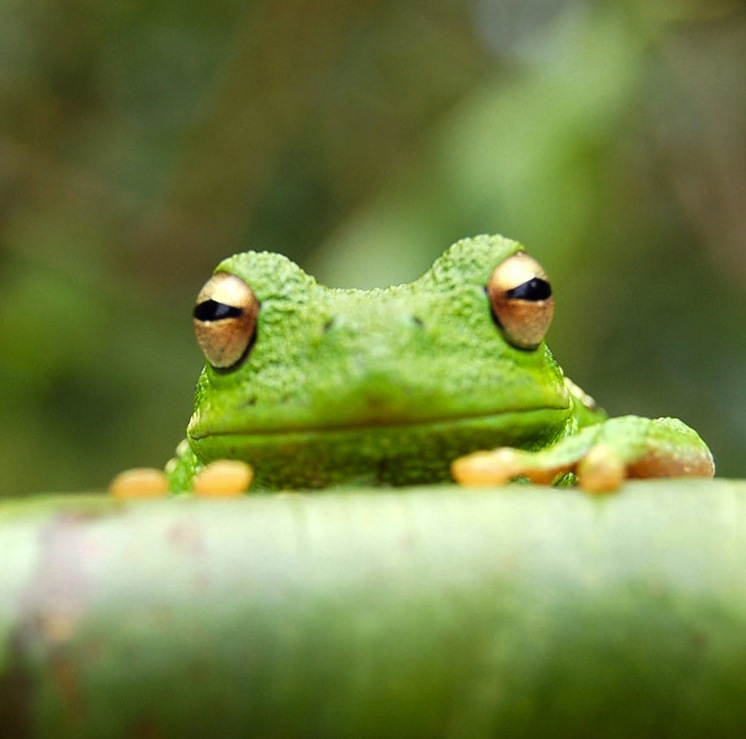
\includegraphics[width=0.5\textwidth]{frog.jpg}
\caption{\label{fig:frog}This is a figure caption.}
\end{figure}

\begin{table}
\centering
\begin{tabular}{l|r}
Item & Quantity \\\hline
Widgets & 42 \\
Gadgets & 13
\end{tabular}
\caption{\label{tab:widgets}An example table.}
\end{table}

\subsection{Mathematics}

\LaTeX{} is great at typesetting mathematics. Let $X_1, X_2, \ldots, X_n$ be a sequence of independent and identically distributed random variables with $\text{E}[X_i] = \mu$ and $\text{Var}[X_i] = \sigma^2 < \infty$, and let
$$S_n = \frac{X_1 + X_2 + \cdots + X_n}{n}
      = \frac{1}{n}\sum_{i}^{n} X_i$$
denote their mean. Then as $n$ approaches infinity, the random variables $\sqrt{n}(S_n - \mu)$ converge in distribution to a normal $\mathcal{N}(0, \sigma^2)$.

\subsection{Lists}

You can make lists with automatic numbering \dots

\begin{enumerate}
\item Like this,
\item and like this.
\end{enumerate}
\dots

\bibliography{Mendeley}

\clearpage  % page breaking
\section*{Matlab Code}
\lstinputlisting{Assignment9_Minoo.m}

\end{document}

%
% Please see the package documentation for more information
% on the APA6 document class:
%
% http://www.ctan.org/pkg/apa6
%